\section{The homogeneous electron gas}\label{sec:4.5}

Spread the four valence electrons of each silicon atom uniformly over the crystal, replace the ions by a uniform positive background, and ask where the loss function of this electron gas peaks at long wavelength. The answer is the plasma frequency, $\omega_p = \SI{16.6}{eV}$, and the measured loss peak of silicon in \cref{fig:4-siloss} lies at \SI{16.4}{eV}. A model with no lattice, no gap and no bonds places the main feature of the spectrum within 1.2 percent of the measured peak. The reason is that at long wavelength and high frequency the valence electrons respond collectively, and the details of the crystal matter less than the Coulomb force between them. The electron gas is also the one interacting system in which the independent-particle response and its screened version can be written in closed form, and this is why it serves as the reference model for valence electrons, plasmons and screening.

The model is jellium (\cref{we:2-jellium}) at the valence density of silicon, $\nd_e = \SI{2.00e23}{cm^{-3}}$. Its density parameter, the radius per electron in units of the Bohr radius, is $r_s = 2.0$ (\cref{sec:2.3}), and the free-gas scales of \cref{eq:2.5-fermi} are $k_{\mathrm{F}} = \SI{3.57}{keV}$, $E_{\mathrm{F}} = \SI{12.5}{eV}$ and $v_{\mathrm{F}} = 7.0\times10^{-3}$. In these units the plasma frequency is $\omega_p = 1.33\,E_{\mathrm{F}}$ and the Thomas--Fermi wavevector of \cref{eq:4.4-TF} is $k_{\mathrm{TF}} = 1.15\,k_{\mathrm{F}}$. Both ratios grow with $r_s$, since $k_{\mathrm{TF}}^2/k_{\mathrm{F}}^2 = 4\alpha m_e/(\pi k_{\mathrm{F}}) = 0.663\,r_s$ with $k_{\mathrm{F}} = (9\pi/4)^{1/3}/(r_sa_0)$: the denser the gas, the weaker the Coulomb force compared with the kinetic energy.

\subsection{The independent-particle bubble}

Without the Coulomb interaction the electrons of jellium are free, and the Lehmann representation \cref{eq:4.1-lehmann} of their density response is a sum over the moves of one electron. Take an occupation-number state $|i\rangle$ of plane waves, with the spin included in the label $\vect{k}$. The operator $n_e(\vect{q}) = \sum_{\vect{k}}c^\dagger_{\vect{k}+\vect{q}}c_{\vect{k}}$ of \cref{eq:2.3-nq} moves one electron from $\vect{k}$ to $\vect{k} + \vect{q}$, and the move is possible only if $\vect{k}$ is occupied and $\vect{k} + \vect{q}$ empty. In the resonant term of \cref{eq:4.1-lehmann} the final state $|f\rangle$ is this move, with weight $n_{\vect{k}}(1 - n_{\vect{k}+\vect{q}})$ and energy $E_f - E_i = \xi_{\vect{k}+\vect{q}} - \xi_{\vect{k}}$. In the antiresonant term $n_e(\vect{q})^\dagger$ makes the reverse move, from $\vect{k} + \vect{q}$ to $\vect{k}$, with weight $n_{\vect{k}+\vect{q}}(1 - n_{\vect{k}})$ and energy $\xi_{\vect{k}} - \xi_{\vect{k}+\vect{q}}$. The two terms then share the denominator $\omega + \xi_{\vect{k}} - \xi_{\vect{k}+\vect{q}} + \ii0^+$, and their numerators combine to $n_{\vect{k}}(1 - n_{\vect{k}+\vect{q}}) - n_{\vect{k}+\vect{q}}(1 - n_{\vect{k}}) = n_{\vect{k}} - n_{\vect{k}+\vect{q}}$. The Pauli factors have cancelled: a move into an occupied state appears in both terms with opposite signs. The thermal average of $n_{\vect{k}}$ over the Gibbs state is $n_{\mathrm{F}}(\xi_{\vect{k}})$, and
\begin{equation}
  R^0(\vect{q},\omega) = \frac{1}{\Vol}\sum_{\vect{k}}\frac{n_{\mathrm{F}}(\xi_{\vect{k}}) - n_{\mathrm{F}}(\xi_{\vect{k}+\vect{q}})}{\omega + \xi_{\vect{k}} - \xi_{\vect{k}+\vect{q}} + \ii0^+} ,
  \label{eq:4.5-R0}
\end{equation}
the independent-particle bubble. This is the Matsubara bubble \cref{eq:4.7-bubble} continued to real frequencies, obtained here without imaginary time. Its imaginary part counts the transitions of \cref{eq:2.5-indep}, and by the fluctuation--dissipation theorem it is $-\tfrac12S^0$ at $T = 0$, with the structure factor of \cref{we:4-gas}.

At $T = 0$ the sum is a set of elementary integrals over the Fermi sphere, which \cref{app:D.8} carries out for any complex frequency $z$ in the upper half plane. The result is the Lindhard function~\cite{lindhard1954properties}.
\begin{keyresult}[Lindhard function]
\begin{equation}
  R^0(q,\omega) = -2\mathcal{N}_{\mathrm{F}}\left\{\frac12 + \frac{k_{\mathrm{F}}}{4q}\Bigl[(1 - \nu_+^2)\,\ell(\nu_+) - (1 - \nu_-^2)\,\ell(\nu_-)\Bigr]\right\} ,
  \label{eq:4.5-lindhard}
\end{equation}
with $\nu_\pm = (\omega + \ii0^+)/qv_{\mathrm{F}} \pm q/2k_{\mathrm{F}}$, $\ell(w) = \ln[(w + 1)/(w - 1)]$ on the principal branch and $\mathcal{N}_{\mathrm{F}} = m_ek_{\mathrm{F}}/2\pi^2$ per spin. It is \cref{eq:D.8-Rz} at $z = \omega + \ii0^+$, and it holds with $\omega + \ii0^+$ replaced by any $z$ with $\Imag z > 0$.
\end{keyresult}
Apart from the prefactor $2\mathcal{N}_{\mathrm{F}}$, the response depends on two numbers only, the momentum in units of the diameter of the Fermi sphere, $y = q/2k_{\mathrm{F}}$, and the frequency in units of the largest Doppler shift, $\omega/qv_{\mathrm{F}}$. On the real axis the logarithms take the branch \cref{eq:C.8-branch}, $\ell(\nu + \ii0^+) = \ln|(\nu + 1)/(\nu - 1)| - \ii\pi\,\Theta(1 - |\nu|)$. The real part, \cref{eq:D.8-Re}, keeps the form of \cref{eq:4.5-lindhard} with the logarithms of the moduli. The imaginary part is a sum of steps, and it is nonzero only between the edges
\begin{equation*}
  \omega_+ = qv_{\mathrm{F}} + \frac{q^2}{2m_e}, \qquad \omega_- = \max\Bigl(0,\ \frac{q^2}{2m_e} - qv_{\mathrm{F}}\Bigr) ,
\end{equation*}
the particle--hole continuum of \cref{fig:4-gas}. Inside it, \cref{eq:D.8-Im} is $-\tfrac12$ times the linear and parabolic forms of $S^0$ found by counting transitions in \cref{we:4-gas}, as the fluctuation--dissipation theorem requires. The real part, which counts the same transitions off resonance through their principal values, is the new information.

The static limit and the high-frequency tail of the real part are needed below. At $\omega = 0$ (\cref{app:D.8}),
\begin{equation}
  R^0(q,0) = -2\mathcal{N}_{\mathrm{F}}\,F_{\mathrm{L}}\Bigl(\frac{q}{2k_{\mathrm{F}}}\Bigr), \qquad
  F_{\mathrm{L}}(y) = \frac12 + \frac{1 - y^2}{4y}\ln\Bigl|\frac{1 + y}{1 - y}\Bigr| ,
  \label{eq:4.5-static}
\end{equation}
with the function $F_{\mathrm{L}}$ of \cref{eq:C.8-FL}, which falls from one at $q = 0$ to $\tfrac12$ at $q = 2k_{\mathrm{F}}$ and decays as $4k_{\mathrm{F}}^2/(3q^2)$ at large $q$. At high frequency it is simplest to start again from the sum. Let $\Delta_{\vect{k}} = q^2/2m_e + kqu/m_e$ be the energy of the move, with $u$ the cosine of the angle between $\vect{k}$ and $\vect{q}$, and let $\langle\cdot\rangle$ be the average over the Fermi sphere. Relabeling $\vect{k} \to -\vect{k} - \vect{q}$ in the term with $n_{\vect{k}+\vect{q}}$, as \cref{app:D.8} does, puts \cref{eq:4.5-R0} at $T = 0$ in the form $R^0 = \nd_e\langle 2\Delta_{\vect{k}}/(z^2 - \Delta_{\vect{k}}^2)\rangle$. For $|z| > \omega_+$, the largest $|\Delta_{\vect{k}}|$, the geometric series converges,
\begin{equation}
  R^0(q,z) = \frac{2\nd_e}{z^2}\sum_{j=0}^\infty\frac{\langle\Delta_{\vect{k}}^{2j+1}\rangle}{z^{2j}}
  = \frac{\nd_eq^2}{m_ez^2}\left[1 + \frac{\tfrac35q^2v_{\mathrm{F}}^2 + (q^2/2m_e)^2}{z^2} + \frac{\tfrac37q^4v_{\mathrm{F}}^4 + O(q^6)}{z^4} + O(z^{-6})\right] .
  \label{eq:4.5-moments}
\end{equation}
The averages are elementary. Odd powers of $u$ vanish, and $\langle k^2u^2\rangle = \tfrac15k_{\mathrm{F}}^2$ and $\langle k^4u^4\rangle = \tfrac{3}{35}k_{\mathrm{F}}^4$ from $\langle k^{2n}\rangle = 3k_{\mathrm{F}}^{2n}/(2n + 3)$ and $\langle u^{2n}\rangle = 1/(2n + 1)$. Hence $\langle\Delta\rangle = q^2/2m_e$, $\langle\Delta^3\rangle = (q^2/2m_e)[(q^2/2m_e)^2 + \tfrac35q^2v_{\mathrm{F}}^2]$ and $\langle\Delta^5\rangle = (q^2/2m_e)[\tfrac37q^4v_{\mathrm{F}}^4 + O(q^6)]$. The leading term is the free-particle tail whose coefficient is the f-sum. The coefficients are the odd moments of the energies of the moves, the frequency moments of $S^0$ of \cref{sec:4.3}.

The crystal bubble of \cref{sec:4.6} is computed on a grid of $\vect{k}$ points, over a finite number of bands and with a broadening in place of $\ii0^+$. The closed form \cref{eq:4.5-lindhard} has no such parameters, and the gas is the standard test of the codes that compute it.

\subsection{The random-phase approximation}

The Coulomb interaction enters through the proper response of \cref{sec:4.4}. The random-phase approximation replaces it by the independent-particle bubble,
\begin{equation}
  \tilde R_{ee} \simeq R^0, \qquad
  \varepsilon_{\mathrm{Lin}}(q,\omega) = 1 - v_{\mathrm{C}}(q)\,R^0(q,\omega), \qquad
  R_{ee} = \frac{R^0}{\varepsilon_{\mathrm{Lin}}} ,
  \label{eq:4.5-rpa}
\end{equation}
by \cref{eq:4.4-eps,eq:4.4-dyson}, and $\varepsilon_{\mathrm{Lin}}$ with $R^0$ of \cref{eq:4.5-lindhard} is the Lindhard dielectric function. In this approximation each electron responds as a free particle to the total potential, external plus Hartree, and to nothing else. It drops the hole that exchange and correlation dig around each electron, which makes the potential an electron feels differ from the average Hartree potential; \cref{sec:4.6} puts it back as an exchange--correlation kernel. The name goes back to Bohm and Pines, who derived the collective oscillation from the equation of motion of $n_e(\vect{q})$ by dropping the terms that couple it to density fluctuations at other wavevectors, on the argument that their phases are random and average out~\cite{bohm1953collective}. The approximation is exact to leading order at high density, $r_s \ll 1$, where the kinetic energy dominates and the correlation hole matters least. At $r_s = 2$ it still holds at long wavelength, since at small $q$ the Hartree term $v_{\mathrm{C}}R^0 \propto 1/q^2$ dominates every correction.

In the static limit the random-phase approximation screens a slowly varying potential exactly as Thomas--Fermi theory does, and it corrects that theory at shorter wavelengths. By \cref{eq:4.5-static} and $k_{\mathrm{TF}}^2 = 2e^2\mathcal{N}_{\mathrm{F}}$,
\begin{equation*}
  \varepsilon_{\mathrm{Lin}}(q,0) = 1 + \frac{k_{\mathrm{TF}}^2}{q^2}\,F_{\mathrm{L}}\Bigl(\frac{q}{2k_{\mathrm{F}}}\Bigr) ,
\end{equation*}
and $F_{\mathrm{L}} = 1 - q^2/12k_{\mathrm{F}}^2 + O(q^4)$ recovers \cref{eq:4.4-TF} at $q \ll k_{\mathrm{F}}$. As the wavelength shrinks to the spacing of the electrons, the gas screens less than the local-equilibrium picture of \cref{sec:4.4} assumes, because a potential that varies on the scale $1/k_{\mathrm{F}}$ cannot be followed by a shift of the local Fermi level. At the silicon valence density and the typical momentum transfer $q_0 = \SI{3.73}{keV}$, $\varepsilon_{\mathrm{Lin}}(q_0, 0) = 2.10$ against $\varepsilon_{\mathrm{TF}} = 2.22$, and the screening factor $1/|\varepsilon|^2$ of the static potential is $1/4.41$ rather than $1/4.9$ (\cref{we:4-tf}). At $q = 2k_{\mathrm{F}}$, the momentum that spans the Fermi sphere, $F_{\mathrm{L}}$ has a logarithmic kink (\cref{app:C.8}). In position space it turns the screening cloud around an impurity into a damped oscillation at the wavevector $2k_{\mathrm{F}}$, the Friedel oscillation; in the lattice dynamics of a metal the same kink is the Kohn anomaly.

\begin{limitbox}[Thomas--Fermi screening][lim:4.5a]
A static potential that varies slowly in an electron gas is screened by the dielectric function $\varepsilon_{\mathrm{TF}} = 1 + k_{\mathrm{TF}}^2/q^2$, with $k_{\mathrm{TF}}^2 = 3\omega_p^2/v_{\mathrm{F}}^2$~\cite[Eq.~(S.14)]{hochberg2021determining}.
\par\smallskip
{\centering
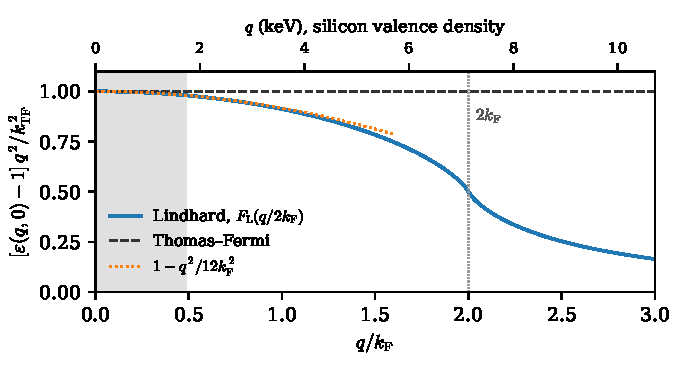
\includegraphics[width=\linewidth]{figures/ch04/limit4_tf.pdf}
\captionof{figure}{Static screening of the electron gas in the random-phase approximation against Thomas--Fermi theory. The induced part of the dielectric function, $[\varepsilon(q,0) - 1]\,q^2/k_{\mathrm{TF}}^2$, is the Lindhard function $F_{\mathrm{L}}(q/2k_{\mathrm{F}})$ (solid) and one for Thomas--Fermi (dashed); dotted, the leading correction $1 - q^2/12k_{\mathrm{F}}^2$. The curve depends on $q/k_{\mathrm{F}}$ alone; the top axis gives $q$ for the silicon valence density, $k_{\mathrm{F}} = \SI{3.57}{keV}$. Gray: $q < 0.49\,k_{\mathrm{F}}$, where the two agree within 2 percent; they differ by 10 percent at $q = 1.06\,k_{\mathrm{F}}$. The kink at $2k_{\mathrm{F}}$ is the edge of the Fermi sphere.}\label{fig:4-tf-limit}
\par}
\smallskip
At $q \gtrsim k_{\mathrm{F}}$ the local-equilibrium picture fails and the gas screens less; beyond $2k_{\mathrm{F}}$ the induced term falls as $1/q^4$ instead of $1/q^2$, and screening dies out.
\end{limitbox}

Static screening at long wavelength is perfect. As $q \to 0$, $\varepsilon_{\mathrm{Lin}}(q, 0) \to \infty$, and an external charge is completely neutralized by the charge it induces: the induced density at $q \to 0$ is $R_{ee}\phi_{\mathrm{ext}} = -(1 - 1/\varepsilon)\,\phi_{\mathrm{ext}}/v_{\mathrm{C}}$, the opposite of the external charge. Through the inverse-moment relation \cref{eq:C.5-screening} this becomes a sum rule for the loss function, $(2/\pi)\int_0^\infty\dd\omega\,L(q,\omega)/\omega = 1 - 1/\varepsilon(q, 0) \to 1$, the perfect-screening sum rule of a metal. At the silicon valence density and $q = 0.1\,k_{\mathrm{F}}$ the right side is 0.9925. In an insulator the same integral is $1 - 1/\varepsilon_\infty$ (\cref{eq:4.4-inverse}), 0.915 for silicon; the gas, with no gap, screens like a metal.

\Cref{fig:4-gasloss}a shows the loss function $L = \Imag(-1/\varepsilon_{\mathrm{Lin}})$ of the gas at $r_s = 2$ over the $(q, \omega)$ plane. Inside the particle--hole continuum, $\varepsilon_2 = -v_{\mathrm{C}}\Imag R^0$ and $L = \varepsilon_2/|\varepsilon_{\mathrm{Lin}}|^2$. At $q \gg k_{\mathrm{F}}$, where $v_{\mathrm{C}}R^0$ is small, $\varepsilon_{\mathrm{Lin}} \to 1$, and the loss function is the free-recoil parabola of \cref{we:4-gas}, centered on $q^2/2m_e$: at short wavelength the electrons scatter one at a time, and screening is irrelevant. At $q \lesssim k_{\mathrm{F}}$ the factor $1/|\varepsilon_{\mathrm{Lin}}|^2$ suppresses the continuum, and the weight moves out of it, into a line above it. Since the f-sum rule fixes the total weight at every $q$, the weight that screening removes from the pairs goes into the line.

\subsection{The plasmon}

The line is the plasma oscillation, and its frequency follows from a classical argument. Displace all the electrons of a slab of jellium by a small distance $s$ along $x$, against the fixed positive background. The two faces of the slab acquire surface charges $\pm e\nd_es$ per unit area, and between them the field, in Heaviside--Lorentz units, is $E = e\nd_es$. Each electron feels the restoring force $-eE$, and $m_e\ddot s = -e^2\nd_es$: the electrons oscillate together at $\omega_p = (e^2\nd_e/m_e)^{1/2}$, the plasma frequency of \cref{eq:4.3-wp}, whatever the size of the slab. No electron moves relative to its neighbors, and no kinetic energy of the Fermi sea enters. At finite wavelength it does, and the random-phase approximation adds it.

A pole of the response with nothing to drive it is a zero of the dielectric function, by \cref{eq:4.4-dyson}. Above the continuum, $\omega > \omega_+$, $\Imag R^0 = 0$ and $\varepsilon_{\mathrm{Lin}}$ is real, so a zero there is a pole of $1/\varepsilon_{\mathrm{Lin}}$ on the real axis, a mode that does not decay. Inserting \cref{eq:4.5-moments} into \cref{eq:4.5-rpa}, with $v_{\mathrm{C}}\nd_eq^2/m_e = \omega_p^2$,
\begin{equation*}
  \varepsilon_{\mathrm{Lin}}(q,\omega) = 1 - \frac{\omega_p^2}{\omega^2}\left[1 + \frac{A}{\omega^2} + \frac{B}{\omega^4} + \dots\right], \qquad
  A = \tfrac35q^2v_{\mathrm{F}}^2 + \Bigl(\frac{q^2}{2m_e}\Bigr)^2, \qquad B = \tfrac37q^4v_{\mathrm{F}}^4 + O(q^6) .
\end{equation*}
Setting it to zero gives $\omega^2 = \omega_p^2 + A\omega_p^2/\omega^2 + B\omega_p^2/\omega^4 + \dots$, which we solve by iteration. At zeroth order $\omega = \omega_p$. Substituting $\omega^2 = \omega_p^2 + A$ on the right, $A\omega_p^2/\omega^2 = A - A^2/\omega_p^2 + O(q^6)$ and $B\omega_p^2/\omega^4 = B/\omega_p^2 + O(q^6)$, so
\begin{keyresult}[Plasmon dispersion in the random-phase approximation]
\begin{equation}
  \omega_{\mathrm{pl}}(q)^2 = \omega_p^2 + \frac35v_{\mathrm{F}}^2q^2 + \Bigl(\frac{1}{4m_e^2} + \frac{12}{175}\,\frac{v_{\mathrm{F}}^4}{\omega_p^2}\Bigr)q^4 + O(q^6) ,
  \label{eq:4.5-dispersion}
\end{equation}
where $\tfrac{12}{175} = \tfrac37 - \tfrac{9}{25}$ collects $B$ and $-A^2$. The plasmon of the electron gas starts at $\omega_p$ and rises quadratically with $q$.
\end{keyresult}
The $q^2$ term is the pressure of the Fermi sea. A classical plasma at temperature $T$ has $3T/m_e$ in place of $\tfrac35v_{\mathrm{F}}^2$. In the degenerate gas the electrons already move at speeds up to $v_{\mathrm{F}}$ at $T = 0$, and $\tfrac35v_{\mathrm{F}}^2$ is three times their mean square velocity along $\vect{q}$, $\langle k^2u^2\rangle/m_e^2 = \tfrac15v_{\mathrm{F}}^2$. Written as $\omega_{\mathrm{pl}} \simeq \omega_p + \alpha_{\mathrm{pl}}q^2/m_e$, the dispersion coefficient is $\alpha_{\mathrm{pl}} = \tfrac35E_{\mathrm{F}}/\omega_p$, 0.45 at the silicon valence density. The expansion converges only outside the continuum, $\omega_{\mathrm{pl}} > \omega_+$, and \cref{fig:4-plasmon-limit} compares it with the exact zero of $\varepsilon_{\mathrm{Lin}}$.

\begin{limitbox}[Plasmon dispersion][lim:4.5b]
In the random-phase approximation the plasmon of an electron gas disperses as $\omega_{\mathrm{pl}}^2 \simeq \omega_p^2 + \tfrac35q^2v_{\mathrm{F}}^2$ and exists up to a cutoff $q_{\mathrm{c}} \simeq \omega_p/v_{\mathrm{F}}$~\cite[Eq.~(171) and the text following it]{kahn2022searches}.
\par\smallskip
{\centering
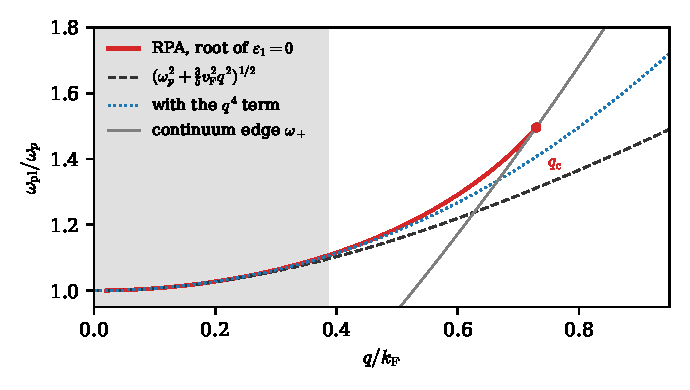
\includegraphics[width=\linewidth]{figures/ch04/limit4_plasmon.pdf}
\captionof{figure}{Plasmon dispersion of the electron gas at $r_s = 2$, the silicon valence density, in the random-phase approximation. Solid: the zero of $\Real\varepsilon_{\mathrm{Lin}}$ above the continuum, computed from \cref{eq:4.5-lindhard}, ending at $q_{\mathrm{c}} = 0.730\,k_{\mathrm{F}}$ where it meets the continuum edge $\omega_+ = qv_{\mathrm{F}} + q^2/2m_e$ (thin line). Dashed: the quadratic formula; dotted: with the $q^4$ term of \cref{eq:4.5-dispersion}. Gray: $q < 0.39\,k_{\mathrm{F}}$, where the quadratic formula is within one percent; there the $q^4$ term reduces the error to below $1.6\times10^{-3}$, and to below $3\times10^{-4}$ for $q < 0.30\,k_{\mathrm{F}}$. The estimate $q_{\mathrm{c}} \simeq \omega_p/v_{\mathrm{F}} = 0.666\,k_{\mathrm{F}}$ is 9 percent low.}\label{fig:4-plasmon-limit}
\par}
\smallskip
Near $q_{\mathrm{c}}$ the series in $q^2$ fails, since the plasmon approaches the pair energies that set its radius of convergence; beyond $q_{\mathrm{c}}$ there is no undamped plasmon.
\end{limitbox}

The weight of the plasmon follows from the slope of $\varepsilon_{\mathrm{Lin}}$ at its zero. Near $\omega_{\mathrm{pl}}$, $\varepsilon_{\mathrm{Lin}} \simeq (\partial\varepsilon_1/\partial\omega)(\omega - \omega_{\mathrm{pl}} + \ii0^+)$, with the $\ii0^+$ carried from $\omega$, and the Sokhotski--Plemelj formula gives
\begin{equation}
  L(q,\omega) = \frac{\pi}{\partial\varepsilon_1/\partial\omega|_{\omega_{\mathrm{pl}}}}\,\delta\bigl(\omega - \omega_{\mathrm{pl}}(q)\bigr) \;\to\; \frac{\pi\omega_p}{2}\,\delta(\omega - \omega_p) \qquad (q \to 0) ,
  \label{eq:4.5-plasmonL}
\end{equation}
since $\varepsilon_1 \to 1 - \omega_p^2/\omega^2$ with slope $2/\omega_p$ at $\omega_p$. At long wavelength the line alone satisfies both sum rules. Its first moment is $(\pi/2)\omega_p^2$, the whole f-sum \cref{eq:4.4-fsumL}, and its inverse moment is $\pi/2$, the whole perfect-screening rule. The continuum, whose weight vanishes as $q \to 0$, has nothing left. By \cref{eq:4.4-SL}, the structure factor at $T = 0$ is then $S = (\pi q^2\omega_p/e^2)\,\delta(\omega - \omega_p)$. Its integral over $\omega$ is $2\pi\nd_eS^{\mathrm{st}}$ by \cref{eq:4.2-static}, and with $e^2\nd_e = m_e\omega_p^2$
\begin{equation*}
  S^{\mathrm{st}}(q) \to \frac{q^2}{2m_e\omega_p} \qquad (q \to 0) .
\end{equation*}
The mean energy $q^2/(2m_eS^{\mathrm{st}})$ of \cref{sec:4.3} is $\omega_p$ at small $q$, and the density fluctuations of the interacting gas vanish as $q^2$, much faster than the $3q/4k_{\mathrm{F}}$ of the free gas. At $q = 0.1\,k_{\mathrm{F}}$ the two are $7.5\times10^{-3}$ and $7.5\times10^{-2}$. The Coulomb force suppresses long-wavelength fluctuations of the charge, since any such fluctuation costs the energy of a plasma oscillation. At finite $q$ the plasmon shares the f-sum with the continuum. Integrating the gridded loss function of \cref{fig:4-gasloss} and adding the weight of \cref{eq:4.5-plasmonL} returns $(\pi/2)\omega_p^2$ to $10^{-5}$ at $q = 0.1\,k_{\mathrm{F}}$ and $0.5\,k_{\mathrm{F}}$; the plasmon carries $1 - 4\times10^{-5}$ of it at $0.1\,k_{\mathrm{F}}$ and 0.957 at $0.5\,k_{\mathrm{F}}$.

The plasmon cannot decay as long as no electron--hole pair has its energy and momentum, that is, as long as $\omega_{\mathrm{pl}}(q) > \omega_+(q)$. The dispersion rises as $q^2$ from $\omega_p$, while the continuum edge rises linearly from zero, and the two meet at the momentum $q_{\mathrm{c}}$ defined by $\varepsilon_{\mathrm{Lin}}(q_{\mathrm{c}}, \omega_+(q_{\mathrm{c}})) = 0$. A rough estimate sets $\omega_+ \simeq qv_{\mathrm{F}}$ equal to $\omega_p$, $q_{\mathrm{c}} \simeq \omega_p/v_{\mathrm{F}}$. At $r_s = 2$ the exact root is $q_{\mathrm{c}} = 0.730\,k_{\mathrm{F}} = \SI{2.60}{keV}$, at $\omega_{\mathrm{pl}} = \SI{24.8}{eV}$; the estimate is $0.666\,k_{\mathrm{F}}$. Beyond $q_{\mathrm{c}}$, $\varepsilon_2 \ne 0$ where $\varepsilon_1$ vanishes, the zero of $\varepsilon_{\mathrm{Lin}}$ continued below the real axis moves into the lower half plane, and the plasmon becomes a resonance of the kind described in \cref{sec:4.1}, with a width that grows quickly with $q$. Its energy goes into single electron--hole pairs. This is Landau damping, named after the analogous damping of waves in a classical plasma by particles that move with the wave.

\begin{figure}[tbp]
  \centering
  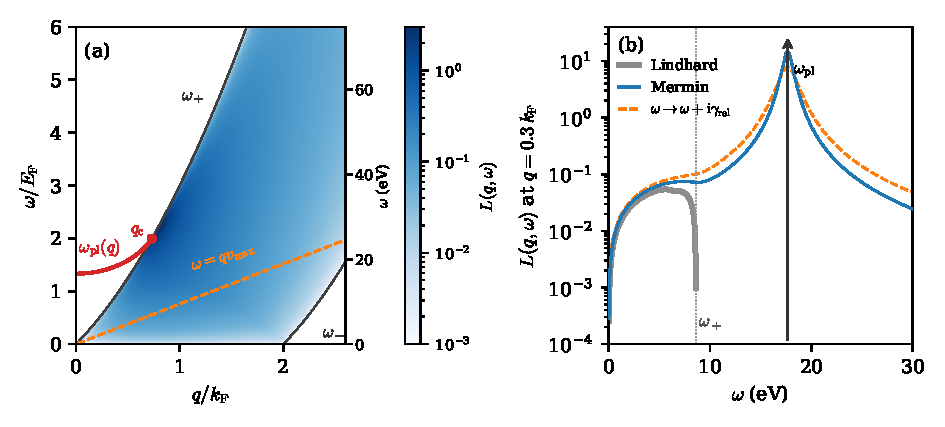
\includegraphics[width=\linewidth]{figures/ch04/fig4_6.pdf}
  \caption{Loss function of the electron gas at $r_s = 2$, the valence density of silicon ($k_{\mathrm{F}} = \SI{3.57}{keV}$, $E_{\mathrm{F}} = \SI{12.5}{eV}$, $\omega_p = \SI{16.6}{eV}$), in the random-phase approximation at $T = 0$. (a) $L(q,\omega) = \Imag[-1/\varepsilon_{\mathrm{Lin}}]$, logarithmic color scale, inside the particle--hole continuum bounded by $\omega_\pm$ (thin lines); the right axis gives $\omega$ in eV. Red: the undamped plasmon $\omega_{\mathrm{pl}}(q)$, a delta function in $L$, drawn as a line up to $q_{\mathrm{c}} = 0.730\,k_{\mathrm{F}}$ (dot), where it enters the continuum and is Landau damped. Dashed: the largest energy a dark-matter particle can deposit at momentum $q$, $\omega = qv_{\mathrm{max}}$ with $v_{\mathrm{max}} = 0.379\,v_{\mathrm{F}}$; it stays below the plasmon at every $q$. (b) $L$ at $q = 0.3\,k_{\mathrm{F}}$ on a logarithmic scale. Thick gray: Lindhard, with the continuum ending at $\omega_+$ and the plasmon as a delta function (arrow, at \SI{17.65}{eV}). Solid: the Mermin function with $\gamma_{\mathrm{rel}} = \SI{1}{eV}$, an illustrative relaxation rate. Dashed: the naive substitution $\omega \to \omega + \ii\gamma_{\mathrm{rel}}$ in $R^0$ with the same rate. Its plasmon peak is twice as wide, and its tail between the continuum and the plasmon is up to 1.7 times higher.}
  \label{fig:4-gasloss}
\end{figure}

In \cref{fig:4-gasloss}a the plasmon line enters the continuum at $q_{\mathrm{c}}$, where the loss function of the continuum is largest. From there a broad Landau-damped ridge continues toward the free-recoil parabola. Dark matter samples the low-energy corner of the continuum, where the electrons near the Fermi surface absorb the energy and the factor $1/|\varepsilon_{\mathrm{Lin}}|^2$ screens it. At small $q$ and $\omega \ll qv_{\mathrm{F}}$ the corner has a simple form. There $\varepsilon_2 = (e^2/q^2)\,m_e^2\omega/(2\pi q)$ from the linear form of $\Imag R^0$, and $\varepsilon_1 \simeq k_{\mathrm{TF}}^2/q^2 \gg \varepsilon_2$, so
\begin{equation*}
  L(q,\omega) \simeq \frac{\varepsilon_2}{\varepsilon_1^2} = \frac{e^2m_e^2}{2\pi k_{\mathrm{TF}}^4}\,q\,\omega \qquad (q \ll k_{\mathrm{F}},\ \omega \ll qv_{\mathrm{F}}) ,
\end{equation*}
linear in both $q$ and $\omega$, and suppressed by the fourth power of the screening wavevector. At the typical momentum transfer $q_0$ and the largest energy $q_0v_{\mathrm{max}} = \SI{9.88}{eV}$, the full Lindhard function yields $|\varepsilon_{\mathrm{Lin}}|^2 = 3.96$ and $L = 0.183$: dynamic screening at the energy deposited is slightly weaker than the static estimate of \cref{we:4-tf}.

\subsection{Collisions and the Mermin function}

In a real metal, or a doped semiconductor, the electrons scatter off impurities and phonons at some rate $\gamma_{\mathrm{rel}}$, and the sharp edges of the Lindhard function and its undamped plasmon are smeared on that scale. The obvious way to include the collisions is to give the frequency an imaginary part, $\omega \to \omega + \ii\gamma_{\mathrm{rel}}$, in $R^0$. This substitution is equivalent to letting the electrons relax toward the uniform equilibrium state at the rate $\gamma_{\mathrm{rel}}$. It has an unphysical consequence: the excess density at a crest of the disturbance decays at that rate even when no current flows to carry it away. Electrons are destroyed at the crests and created in the troughs. Collisions with impurities and phonons conserve the number of electrons, and they relax the shape of the distribution at each point while leaving the number of electrons there unchanged. Mermin~\cite{mermin1970lindhard} therefore let the electrons relax toward a local equilibrium that has, at each instant, the same density as the disturbed gas. \Cref{app:D.9} solves the equation of motion of the one-electron density matrix with this relaxation term and finds the response $\delta\nd_e/\phi = R^{\mathrm{Mer}}$, which in the random-phase approximation gives the Mermin dielectric function.
\begin{keyresult}[Mermin dielectric function]
\begin{equation}
  \varepsilon_{\mathrm{Mer}}(q,\omega) = 1 + \frac{(1 + \ii\gamma_{\mathrm{rel}}/\omega)\,\bigl[\varepsilon_{\mathrm{Lin}}(q,\omega + \ii\gamma_{\mathrm{rel}}) - 1\bigr]}{1 + (\ii\gamma_{\mathrm{rel}}/\omega)\,\bigl[\varepsilon_{\mathrm{Lin}}(q,\omega + \ii\gamma_{\mathrm{rel}}) - 1\bigr]/\bigl[\varepsilon_{\mathrm{Lin}}(q,0) - 1\bigr]} ,
  \label{eq:4.5-mermin}
\end{equation}
with $\varepsilon_{\mathrm{Lin}}$ at the complex frequency $\omega + \ii\gamma_{\mathrm{rel}}$ from \cref{eq:4.5-lindhard} and its static value from \cref{eq:4.5-static}. It conserves the number of electrons at every $q$ and $\omega$, and it reduces to $\varepsilon_{\mathrm{Lin}}$ as $\gamma_{\mathrm{rel}} \to 0$.
\end{keyresult}
This is \cref{eq:D.9-eps}, Mermin's form~\cite{mermin1970lindhard}, and Refs.~\cite[Eq.~(19)]{knapen2021dark} and \cite[Eq.~(168)]{kahn2022searches}, where the rate is written $\varGamma$ and $\varGamma_p$. Analyticity of $R^0(q, z + \ii\gamma_{\mathrm{rel}})$ in the upper half plane does not by itself exclude a zero of the denominator there. \Cref{app:D.9} shows that relaxation toward local equilibrium has no growing free mode, so the Mermin response has no pole in the upper half plane and is causal.

In the continuity equation \cref{eq:D.9-continuity}, the naive substitution adds a source term, $-\ii\gamma_{\mathrm{rel}}$ times the density, and Mermin's reference state makes this term vanish identically. A static potential and the long-wavelength limit tell the two prescriptions apart, as \cref{app:D.9} works out; the f-sum rule does not. For a static potential, $\omega \to 0$ at fixed $\gamma_{\mathrm{rel}}$, $\varepsilon_{\mathrm{Mer}} \to \varepsilon_{\mathrm{Lin}}(q, 0)$: a static potential leaves the electrons in equilibrium in that potential, with or without collisions, so the static screening, perfect screening included, is that of the collisionless gas. The naive substitution yields $\varepsilon_{\mathrm{Lin}}(q, \ii\gamma_{\mathrm{rel}})$ instead; at $q = 0.3\,k_{\mathrm{F}}$ and $\gamma_{\mathrm{rel}} = \SI{1}{eV}$ in the silicon-density gas it is 12.8 against the correct 15.7. At long wavelength, $q \to 0$ at fixed $\omega$, the Mermin function becomes the Drude dielectric function,
\begin{equation*}
  \varepsilon_{\mathrm{Mer}} \to 1 - \frac{\omega_p^2}{\omega(\omega + \ii\gamma_{\mathrm{rel}})} = 1 + \frac{\ii\sigma_{\mathrm{cond}}}{\omega}, \qquad
  \sigma_{\mathrm{cond}}(\omega) = \frac{\omega_p^2}{\gamma_{\mathrm{rel}} - \ii\omega} ,
\end{equation*}
by \cref{eq:4.4-sigma}, with the dc conductivity $\omega_p^2/\gamma_{\mathrm{rel}}$ of a metal whose electrons are scattered at the rate $\gamma_{\mathrm{rel}}$. The naive substitution leads to $1 - \omega_p^2/(\omega + \ii\gamma_{\mathrm{rel}})^2$, which tends to $1 + \omega_p^2/\gamma_{\mathrm{rel}}^2$ as $\omega \to 0$: no dc current and a finite static dielectric constant, the response of an insulator. Both functions are analytic in the upper half plane and both fall off as $\omega_p^2/\omega^2$, so both obey \cref{eq:4.4-fsumL} by the argument of \cref{app:C.5}.

At $q \to 0$ the Drude form puts the whole loss function in one Lorentzian line~\cite[Eq.~(172)]{kahn2022searches},
\begin{equation*}
  L(0,\omega) = \frac{\omega_p^2\,\gamma_{\mathrm{rel}}\,\omega}{(\omega^2 - \omega_p^2)^2 + \gamma_{\mathrm{rel}}^2\omega^2} .
\end{equation*}
It is the damped oscillator of \cref{we:4-oscillatorL} with $\omega_{\mathrm{res}} = \omega_p$, no gap, and $\gamma_{\mathrm{rel}}$ in the role of $\varGamma_{\mathrm{w}}$. The plasmon now has the full width $\gamma_{\mathrm{rel}}$, and below it the loss function has a tail, $L \simeq \gamma_{\mathrm{rel}}\omega/\omega_p^2$ for $\omega \ll \omega_p$, linear in $\omega$ down to zero frequency. The naive substitution puts the pole at $\pm\omega_p - \ii\gamma_{\mathrm{rel}}$, with twice the width and twice the tail, $2\gamma_{\mathrm{rel}}\omega/\omega_p^2$. \Cref{fig:4-gasloss}b compares the three functions at $q = 0.3\,k_{\mathrm{F}}$. For a dark-matter particle, which deposits energies far below the plasmon, the tail is the part that matters. It is weight that the Lindhard function does not have at small $q$, and whether a real material has it depends on the material~\cite{hochberg2021determining,kahn2022searches}.

In practice the Mermin function is used as a fitting form. The plasmon of silicon has a width of a few eV, but it does not come from collisions: the plasmon decays into interband electron--hole pairs, as \cref{we:4-siplasmon} shows. A rate $\gamma_{\mathrm{rel}}$ fitted to that width is a parameter of the fit, not a collision rate. The Mermin oscillator method of Ref.~\cite[Eqs.~(20) and (21)]{knapen2021dark} writes the measured optical loss function as a sum of Mermin terms,
\begin{equation*}
  L(q,\omega) = \sum_i A_i(q)\,\Imag\bigl[-1/\varepsilon_{\mathrm{Mer}}(q,\omega;\omega_{p,i},\gamma_i)\bigr]\,\Theta(\omega - \omega_{\mathrm{edge},i}) .
\end{equation*}
Each term has its own plasma frequency $\omega_{p,i}$, rate $\gamma_i$ and onset $\omega_{\mathrm{edge},i}$. The parameters are fitted at $q = 0$, and the Mermin function carries each term to finite $q$. The amplitudes $A_i(q)$ are rescaled at each $q$ so that every term keeps its share of the f-sum. The step functions remove the weight below the gap that a single gas would put there. The method is a way to extrapolate optical data to the momentum transfers of dark-matter scattering while keeping the sum rules; the physics of the extrapolation is that of the gas.

\begin{workedexample}{The silicon valence electrons as an electron gas}\label{we:4-siplasmon}
Treat the four valence electrons per atom of silicon as jellium at $\nd_e = \SI{2.00e23}{cm^{-3}}$, $r_s = 2.0$. The plasma frequency is $\omega_p = \SI{16.6}{eV}$ (\cref{eq:4.3-wp}), and by \cref{eq:4.5-dispersion} the plasmon disperses as $\omega_{\mathrm{pl}} \simeq \omega_p + 0.45\,q^2/m_e$, up to $q_{\mathrm{c}} = \SI{2.60}{keV}$ and $\omega_{\mathrm{pl}} = \SI{24.8}{eV}$. The measured loss function at $q \to 0$ (\cref{fig:4-siloss}) peaks at \SI{16.4}{eV}, and $\varepsilon_1$ crosses zero at \SI{16.3}{eV}; the gas places the zero 1.9 percent higher.

\emph{Position.} Near \SI{16}{eV} the valence electrons of silicon respond almost as if they were free. In the tabulated data, 87 percent of their f-sum weight $\int\omega\varepsilon_2\,\dd\omega$ lies below \SI{16.3}{eV}, at a root-mean-square energy of \SI{6.5}{eV}, in the interband transitions of \cref{fig:4-siloss}a. A transition at an energy $\omega_i$ well below $\omega$ contributes to $\varepsilon_1$ as an oscillator driven above its resonance, $-f_i/(\omega^2 - \omega_i^2) \simeq -(f_i/\omega^2)(1 + \omega_i^2/\omega^2)$, which is the free-electron term with a correction of order $(\omega_i/\omega)^2 \approx 0.16$. The slope of the data confirms the picture: at the zero, $\partial\varepsilon_1/\partial\omega = \SI{0.128}{eV^{-1}}$, against $2\omega_p^2/\omega^3 = \SI{0.127}{eV^{-1}}$ for the gas. The correction from binding has the sign that pushes the zero up; if all the weight were in one oscillator at \SI{5.08}{eV}, the resonance of the single-oscillator model, the zero would move to $\bar E = \SI{17.4}{eV}$ (\cref{we:4-oscillatorL}). The remaining weight, 9.4 percent between \SI{16.3}{eV} and \SI{40}{eV} and the rest above, lies above the plasmon and contributes positively to $\varepsilon_1$, which pulls the zero down. The two shifts nearly cancel.

\emph{Width.} In the gas at $q \to 0$ the plasmon cannot decay, since the continuum shrinks to $\omega < qv_{\mathrm{F}} \to 0$. In silicon, vertical interband transitions exist at all energies up to well above \SI{16}{eV}, and at the zero of $\varepsilon_1$ the data have $\varepsilon_2 = 0.224$. Near the zero $L = \varepsilon_2/(\varepsilon_1^2 + \varepsilon_2^2)$ with $\varepsilon_1 \simeq (\partial\varepsilon_1/\partial\omega)(\omega - \omega_{\mathrm{pl}})$, a Lorentzian of full width $2\varepsilon_2/(\partial\varepsilon_1/\partial\omega) = \SI{3.5}{eV}$, against the measured \SI{3.66}{eV}. The plasmon of silicon decays into interband electron--hole pairs: the crystal potential supplies the momentum that, in the gas, only $q > q_{\mathrm{c}}$ could provide. A Mermin function with $\gamma_{\mathrm{rel}} = \SI{3.66}{eV}$ reproduces the line: at $q \to 0$ its peak height is $\omega_p/\gamma_{\mathrm{rel}} = 4.54$, against the measured 4.5. Its tail, however, is $L = 0.042$ at \SI{3}{eV}, 14 times the measured $3.1\times10^{-3}$, and it continues below the gap, where silicon absorbs nothing, just as the single oscillator of \cref{we:4-oscillatorL} did.

\emph{Dark matter.} The plasmon is out of reach. A halo particle deposits at most $qv_{\mathrm{max}}$, and with $v_{\mathrm{max}} = 0.379\,v_{\mathrm{F}}$ the line $\omega = qv_{\mathrm{max}}$ reaches $\omega_p = \SI{16.6}{eV}$ only at $q = \omega_p/v_{\mathrm{max}} = \SI{6.26}{keV} = 1.75\,k_{\mathrm{F}}$, far beyond $q_{\mathrm{c}}$, where the gas has no plasmon left (\cref{fig:4-gasloss}a). The plasmon, which carries most of the weight at small $q$, is kinematically inaccessible~\cite{kahn2022searches}. The particle samples the low-energy side of the loss function, at a few eV, where the gas and the crystal differ most. The gas has a continuum down to $\omega = 0$, screened by $|\varepsilon_{\mathrm{Lin}}|^2 \approx 4$ at $q_0$, while silicon has a gap, interband peaks, and an optical loss function of $3.1\times10^{-3}$ at \SI{3}{eV}. The electron gas is a good model of the peak that holds most of the f-sum and a poor one of the corner that sets the rate. Its use in the dark-matter literature is accordingly limited to energies well above the gap, between about 5 and \SI{15}{eV}, where it describes the computed spectrum of silicon and germanium fairly well~\cite{kahn2022searches}.
\end{workedexample}
